\documentclass[tikz]{standalone}
\usepackage{pgfplots}
\pgfplotsset{compat=newest}
\usepgfplotslibrary{
  groupplots
}
\begin{document}
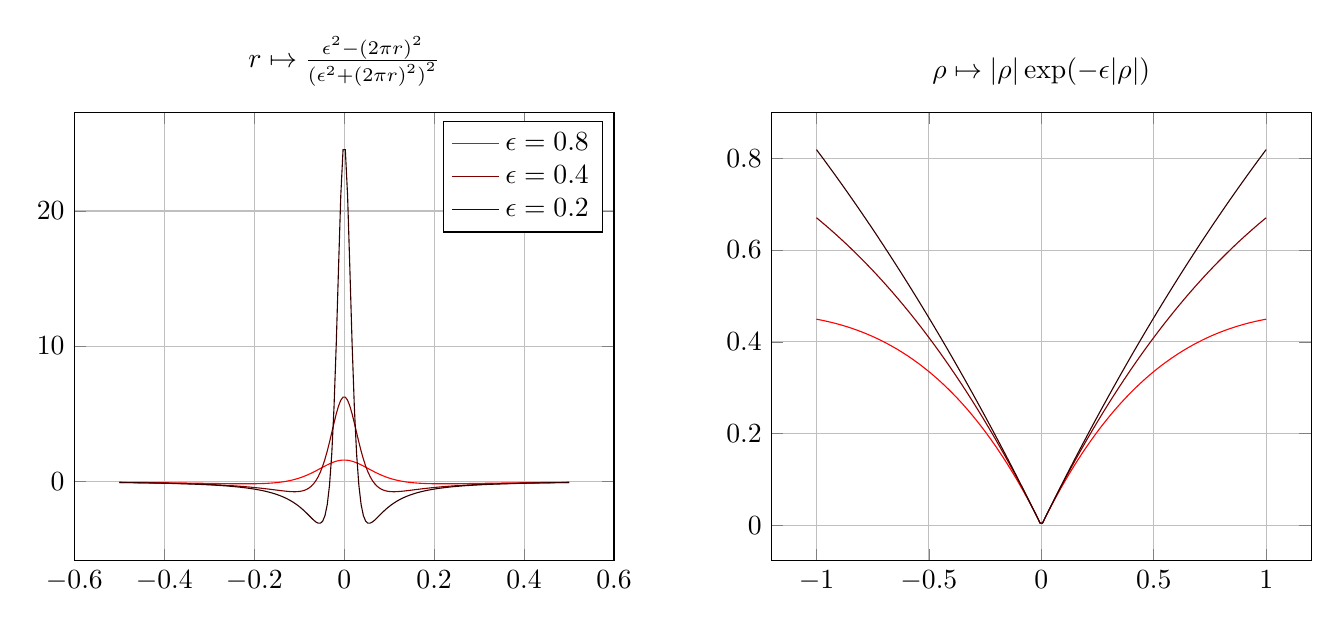
\begin{tikzpicture}
	\begin{groupplot}[
		group style={group size=2 by 1, horizontal sep=2cm},
	]
	\nextgroupplot[
		domain=-0.5:.5,
		samples=200,
		title={\( r \mapsto \frac{\epsilon^2 - {(2\pi r)}^2}{{(\epsilon^2 + {(2\pi r)}^2)}^2} \)},
		grid=major,
	]
	\def\ee{0.8}
	\addplot [red] {(\ee^2 - (2*pi*x)^2) / (\ee^2 + (2*pi*x)^2)^2};
	\def\ee{0.4}
	\addplot [red!50!black] {(\ee^2 - (2*pi*x)^2) / (\ee^2 + (2*pi*x)^2)^2};
	\def\ee{0.2}
	\addplot [red!20!black] {(\ee^2 - (2*pi*x)^2) / (\ee^2 + (2*pi*x)^2)^2};
	\legend{\( \epsilon = 0.8 \),\( \epsilon = 0.4 \),\( \epsilon = 0.2 \)}
	\nextgroupplot[
		domain=-1:1,
		samples=200,
		title={\( \rho \mapsto |\rho| \exp(-\epsilon|\rho|)\)},
		grid=major,
	]
	\def\ee{0.8}
	\addplot [red] {abs(x) * e^(-\ee * abs(x))};
	\def\ee{0.4}
	\addplot [red!50!black] {abs(x) * e^(-\ee * abs(x))};
	\def\ee{0.2}
	\addplot [red!20!black] {abs(x) * e^(-\ee * abs(x))};
\end{groupplot}
\end{tikzpicture}
\end{document}
